
% \begin{figure}
%   \centering
%   \begin{tikzpicture}[
%     level distance=1.5cm,
%     every node/.style={draw, rectangle, rounded corners=3pt, align=center, text width=3cm},
%     edge from parent/.style={draw, ->, >=angle 60, thick}, % Set arrowhead style here
%     sibling distance=4cm,
%     level 1/.style={sibling distance=8cm},
%     level 2/.style={sibling distance=4cm}
%   ]

%   \node {Offline RL}
%     child { node {Model-Free} }
%     child { node {Model-Based}
%       child { node {Robust}
%         child { node {Uncertainty Quantification} }
%         child { node {No Uncertainty Quantification} }
%       }
%       child { node {Adaptive} }
%     };
%   \end{tikzpicture}
%   \caption{Model-Based Offline Reinforcement Learning Taxonomy}
%   \label{fig:your-label}
% \end{figure}

\begin{figure}
    \centering
    \adjustbox{scale=0.75}{
    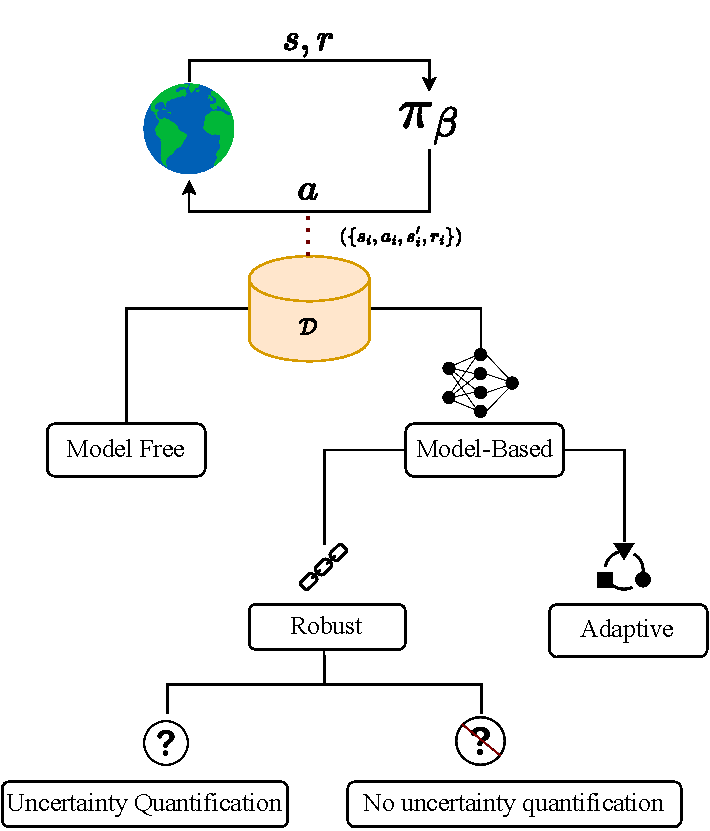
\includegraphics[width=0.7\textwidth]{4_Taxonomy/tax_diag.pdf}}
    \caption{Offline Reinforcement Learning Taxonomy}
    \label{fig:taxonomy}
\end{figure}

Considering the exponential rise in publications in the offline RL field in the past few years, researchers and practitioners must navigate various novel approaches while maintaining a clear contextual comprehension. Levine et al., in their seminal paper on offline RL, outline the theoretical and functional aspects of offline RL methods and highlight the diverse approaches and challenges within the field. Recently, Prudencio et al. expanded the coverage of Levine et al.’s work by introducing a novel taxonomy to categorize offline RL from algorithmic, dataset, and performance perspectives. They comprehensively compare various methodologies, spanning model-free and model-based approaches, importance sampling, regularization, uncertainty estimation, trajectory optimization, one-step methods, and imitation learning algorithms. In their dataset analysis, they present definitions that describe the difficulties posed by the inherent attributes of evaluation datasets across standard RL benchmarking suites. The most notable and relevant to this study is the Suboptimal Dataset (SD) characteristic. SDs are essential in testing an algorithm’s generalizability as they evaluate a learned policy’s ability to filter out poor behaviors from the dataset and improve upon the underlying suboptimal behavioral policy. The model-based offline RL papers analyzed in this study mostly evaluate model performance in D4RL’se in D4RL’s Gym-MuJoCo suite- a standard benchmark containing SD datasets. 

This study narrows the scope of Prudencio et al.’s work to specific subproblems. We lean on their work in formulating a taxonomy for model-based methods but specifically evaluate them from a generalizability perspective. We divide offline RL based on the presence of learning dynamics models into model-free and model-based methods. Other works also consider trajectory optimization or planning methods as valid splits. \autoref{fig:taxonomy} outlines the categories in our taxonomy. First, a behavioural policy interacts with the world and its interactions are stored in the static dataset $\mathcal{D}$. Then, we provide a hierarchical overview on the different policy learning approaches which can leverage the offline dataset. Someone et al. (assessing generalization in RL paper) evaluate the generalizability of model-free methods and state that policy learning is of two types- robust and adaptive. 

\subsection{Robust and Adaptive Policy Learning}
Robust policy learning aims to learn a policy resilient to environmental variations. In contrast, adaptive methods train the policy to be adaptive and flexible when environmental dynamics, rewards, and objectives alter during evaluation. Most robust RL methods implement some form of conservatism during policy learning. This is especially crucial in offline RL, where exploitation of the poor coverage of the state-action space can degrade real-world performance. On the other hand, adaptive policy learning leverages test data to calibrate the learned policy to new tasks or environments. The same distinction applies to the paradigm of model-based learning, which we use in this taxonomy. Policy learning algorithms are primarily designed to be robust. Within this framework, we further split the robust category into two subgroups: methods that incorporate uncertainty quantification and those that do not. 

\subsection{Uncertainty Estimation}
Model-based approaches must balance exploring and exploiting out-of-
distribution (OOD) areas by learning a dynamics model capable of providing guidance on the next action based on the agent’s current state and past state visitations while conveying confidence in its predictions. The leading method of encoding confidence regarding the agent’s actions is through uncertainty estimation. Uncertainty estimation approximates the trust in the model’s behavior by quantifying the disagreement between its learned transition probability estimates and the actual transition probabilities. Based on this estimate, a penalty is enforced to ensure conservatism (typically in the reward function or dynamics model), which prevents the policy from leaving the support of the offline dataset. Estimating model uncertainty can be challenging due to certain limitations. These limitations include the need for strong assumptions regarding access to a model error oracle- which provides an upper bound on model error for any state-action tuple [Combo paper]. Another limitation is the reliance on neural networks, which may propagate poor uncertainty estimates during model learning. 

A separate branch of model-based methods that forgo uncertainty quantification during model learning by substituting it with regularization or Q-learning approaches has surfaced. These methods rely on behavioral regularization, conservative Q -learning adapted to utilize a dynamics model, generating imaginative trajectories, or adversarial model training to address the aforementioned limitations. Although accurate uncertainty modeling is desirable to improve model transparency, it may not always be feasible. In some cases, avoiding uncertainty estimation reduces computational complexity and improves training stabilization to produce more efficient algorithms. 








 








